\chapter{Test Functions for Optimization}
\label{chap:test_functions}
  This appendix contains the test functions used in the numerical experiments in 
  \vref{chap:case_study_real_function_optimization}.

  \section{Rastrigin Function}
  \label{sec:test_functions:rastrigin}
    The Rastrigin function is a non-convex function used as a performance test problem for 
    optimization algorithms.
    It is a typical example of non-linear multimodal function.
    It was first proposed by Rastrigin in 1974.\footnote{
      Rastrigin, L. A. \enquote{Systems of extremal control.} Mir, Moscow (1974).
    }

    \begin{definition}[Rastrigin Function]
      \label{def:test_functions:rastrigin}
      The \emph{Rastrigin function}, \(f: \mathbb{R}^n \rightarrow \mathbb{R}\), is defined as:

      \begin{equation}
        \label{eq:test_functions:rastrigin}
        f(\mathbf{x}) = An + \sum_{i=1}^{n} \left[ \mathbf{x}_i^2 - A\cos(2\pi \mathbf{x}_i) \right]
      \end{equation}
        
      where:

      \begin{itemize}
        \item \(n\) is the number of dimensions.
        \item \(\mathbf{x}\) is a vector of \(n\) real values.
      \end{itemize}
    \end{definition}

    The global minimum of the Rastrigin function is \(f(\mathbf{x}^*) = 0\) at \(\mathbf{x}^* = 
    (0, \ldots, 0)\).
    The function has many local minima, which are regularly distributed.
    The \(A\) parameter controls the depth of the local minima.
    The function is usually evaluated on the hypercube \(\mathbf{x} \in [-5.12, 5.12]^n\).
    A contour plot and a surface plot of the Rastrigin function for \(n = 2\) are shown in
    \vref{fig:test_functions:rastrigin}.

    \begin{figure}[ht!]
      \centering
      \begin{subfigure}[b]{0.4\textwidth}
        \centering
        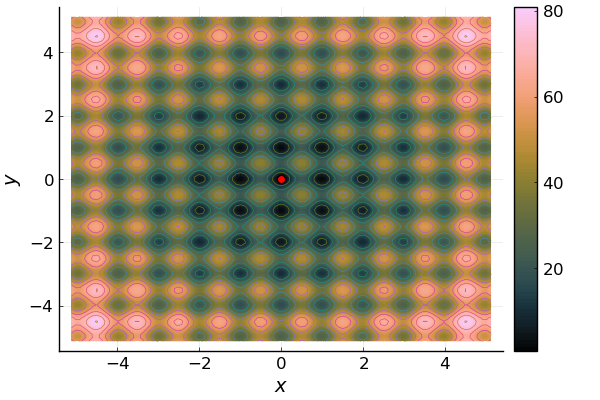
\includegraphics[width=\textwidth]{img/test_functions/rastrigin_contour.png}
      \end{subfigure}
      \begin{subfigure}[b]{0.4\textwidth}
        \centering
        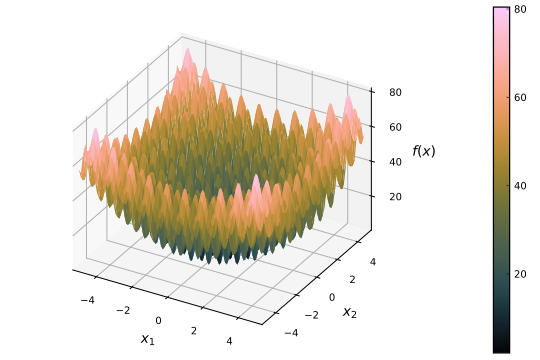
\includegraphics[width=\textwidth]{img/test_functions/rastrigin_surface.png}
      \end{subfigure}
      \caption{Rastrigin Function for \(n = 2\)}
      \label{fig:test_functions:rastrigin}
    \end{figure}
